\subsection{Discuss the ground states of larger atoms (up to Ne) by using Hund's first rule. Explain the general structure of the periodic table of elements (e.g. transition metals) based on the population of the electronic shells.}


For at beskrive opbygningen af det periodiske system samt grundtilstanden for større atomer, så er det vigtigt at kende til Hunds første regel, og dermed også kende til Paulis udelukkelsesprincip.

\paragraph{Hunds første regel:} ''For enhver atomgrundtilstand vil det totale elektronspin have den maksimale værdi tilladt af Paulis undelukkelsesprincip.'' \footnote{For fuldstændighed, så nævnes her Hunds anden og tredje regel:
\begin{enumerate}
    \setcounter{enumi}{1}
    \item For a given multiplicity, the term with the largest value of the total orbital angular momentum quantum number $L$ has the lowest energy.
    \item For a given term, in an atom with outermost subshell half-filled or less, the level with the lowest value of the total angular momentum quantum number $J$ lies lowest in energy. If the outermost shell is more than halffilled, the level with the highest value of $J$ is lowest in energy.
\end{enumerate}
}

\paragraph{Paulis udelukkelsesprincip:} Basseret på undersøgelser af fler-elektron atomer, observerede Pauli, at de eneste atomtilstanden, som kan observeres i naturen, beskrives ved en totalbølgefunktion ($\Psi = \psi(\Vec{r})\cdot\chi(\Vec{s})$), som er antisymmetrisk under ombytning af elektronerne. En mere teoretisk tilgang til systemer med identiske partikler viser, at dette gør sig gældende ikke kun for elektroner, men for alle fermioner (partiklern med spin $n/2$, for $n\in\mathbb{N}\setminus\{0\}$, som elektroner, protoner og neutroner). Derved bliver Pauli princippet
\begin{quote}
    ''Den totale bølgefunktion for et system med mere end én identisk fermion skal altid være antisymmetrisk under ombytning af disse fermioner.''
\end{quote}
eller
\begin{quote}
    ''En atomtilstand med de tre kvantetal ($n$, $l$, $m_l$) kan maksimalt være optaget af to elektroner med modsat spin-orientering ($m_s = \pm 1/2$).''
\end{quote}
$ $\\\\

\paragraph{Opbygning af det periodiske system:} The ground state electron configuration for heavier atoms can be pieced together in much the same way. Ignoreres frastødningen indbyrdes mellem elektronerne \ldots
\noindent
Idet elektronerne er femioner er de underlagt Paulis udelukkelsesprincip, hvorfor der maksimalt kan være \emph{to} elektroner i enhver orbital -- én spin op og én spin ned, eller mere specifik skal de være i en singlet-konfiguration. Der er $n^2$ hydrogenic bølgefunktioner, som alle vil have den samme energi $E_n$, for et givet hovedkvantetal $n$, så vil $n$-skallen have plads til $2n^2$ elektroner, så for $n=1$ skallen vil der være plads til 2 elektroner, for $n=2$ skallen vil der være plads til 8 elektroner, for $n=3$ skallen vil der være plads til 18 elektroner, osv..

Kvalitativt så ville man se rækkerne i det periodiske system som svarende til at fylde en skal, men som vi kan observere af det periodiske system, så er rækkernes længde hhv. 2, 8, 8, 18, 18, osv. og ikke 2, 8, 18, 32, 50, hvilket de ville være, hvis en række blot var svarende til at fylde en hel skal. Dette skyldes vores antagelse om ignorere interaktionen mellem elektronerne. Dette problem kan vi se allerede i anden skal: Vi ved at med hydrogen og helium, så er $n=1$ skallen fyldt, så for lithium skal der en elektron i $n=2$ skallen. For $n=2$ kan impulsmomentet være $l=0$ eller $l=1$, men hvilken af disse orbitaler vil den tredje elektron lægge sig i? Uden interaktionen mellem elektronerne, da vil disse orbitaler have den samme energi, siden Bohr-energierne er afhængig af $n$ men ikke af $l$.

Interaktionenen mellem elektronerne vil favoritisere det laveste værdier af $l$, hvilket intuitivt kan forståes ved at impulsmomentet ''smider'' elektronen ud i en større bane, og jo længe ud at den kommer, jo mere blokeres kernen af de indre elektroner (effekten hedder på engelsk \emph{screening}), så man kan se det som om at de indre elektroner ser kernen med ladning $Ze$, mens den yderste elektron ser kernen med effektiv ladning $\sim e$, hvorfor de inderste elektroner er bedre bundet, hvorfor disse må have en lavere energi; altså må energien stige med stigende impulsmoment $l$. Så i eksemplet fra før vil lithium lægge sig s-obitalen ($l=0$), hvilket også beryllium vil, men som den næste skal bohr gøre brug af p-obitalen ($l=1$), hvilket de resterende grundstoffer op til og med neon også skal. Per Hunds første regel vil elektronerne forsøge at maksimere spinet, hvorfor de i p-obitalerne vil lægge sig i hver deres og alle være spin-op ($m_s = 1/2$), indtil der ikke er flere ledige p-obitaler i skal $n=2$, hvilket kan ses på \cref{fig:Q13_FyldningAfDeInderstseToSkaller}.

\begin{figure}[!h]
    \centering
    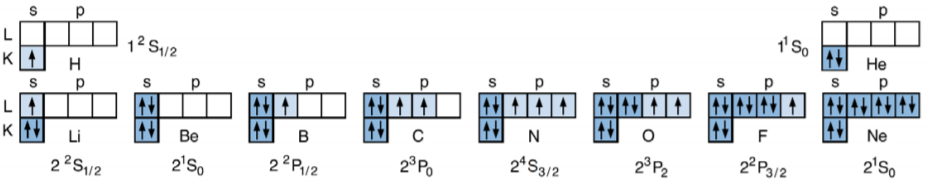
\includegraphics[width=\textwidth]{Q13/images/FirstTwoShellsElectronicSpinConfiguration.PNG}
    \caption{Princippet for opbygning af elektronkofigurationen for grundtilstanden for de første ti grundstoffer. Pilen angiver elektronens spin med $m_s = \pm 1/2$. I tilstanden, hvor der kun er én enkelt elektron kan kvantetallet for dennes spin være både $m_s = \pm 1/2$, mens den ellers vil være bestemt af den anden elektron i tilstanden, jvf. Paulis udelukkelsesprincip.}
    \label{fig:Q13_FyldningAfDeInderstseToSkaller}
\end{figure}

\paragraph{Obitalnavne:} Se \cref{tab:Q13_ImpulsmomenterOrbitalerOgDeresNavne}.
\begin{table}[!h]
    \centering
    \begin{tabular}{|c|c|c|c|c|c|c|c|c|c|c|c|}
        \hline
        $l=$ & 0 & 1 & 2 & 3 & 4 & 5 & 6 & 7 & 8 & \ldots\\
        \hline
        \textbf{Orbital} & s & p & d & f & g & h & i & k & l & \ldots \\
        \hline
        \textbf{Navn} & sharp & principal & diffuse & fundamental & & & & & &\\
        \hline
    \end{tabular}
    \caption{Impulsmomenter med tilhørenden orbitaler og deres obitalnavne.}
    \label{tab:Q13_ImpulsmomenterOrbitalerOgDeresNavne}
\end{table}

Nu har vi talt om, hvordan opbygningen af de første ti atomer er, og deres orbitaler fylder op nogenlunde logisk. I tredje skal er opfyldningen af s- og p-orbitalen stadig logisk nok, men efter argon, der fyldte sidste plads i d-orbitalen ville man formode, at man ville fylde elektroner i $3d$-orbitalen, hvilken har plads til 10 elektroner, men dette er ikke tilfældet, og $4s$-orbitaler bliver i stedet fyldt med 2 elektroner først, hvorefter $3d$-orbitalen fyldes op. Dette skyldes, at energiniveauerne her overlapper således, at $4s$-orbitalen faktisk har lavere energi end $3d$-orbitalen. Dette mønster fortsætter gennem det periodiske system, hvorfor man fylder orbitalerne som set på \cref{fig:Q13_FyldningAfSkaller}, og man kan se det i forbindelse med det periodiske system som \cref{fig:Q13_OpfyldningAfSkallerMedPeriodiskSystem}.
\noindent
Hvis det er helt rigtigt, så er der nogle småting ved opfyldningen af grundstoffet lige før (i s-orbitalen) og efter (i d-orbitalen) både lataniderne og aktaniderne, som lige mellem disse to (før og efter) springer ned og fylder med første grundstof fra lataniderne eller aktaniderne (alt efter hvilke grundstoffer, som vi taler om) i f-orbitalen. Dette kan ses af \cref{fig:Q13_FyldningAfSkallerFaktisk}.

\begin{figure}[!h]
    \centering
    \begin{subfigure}[t]{\textwidth}
        \centering
        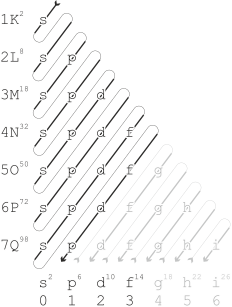
\includegraphics[width=0.5\textwidth]{Q13/images/FyldningAfSkaller3.png}
        \caption{Skallerne fyldes efter følgende møster (med små afvigelser som vist på \cref{fig:Q13_FyldningAfSkallerFaktisk}).}
        \label{fig:Q13_FyldningAfSkaller1}
    \end{subfigure}
    \vfill
    \begin{subfigure}[t]{\textwidth}
        \centering
        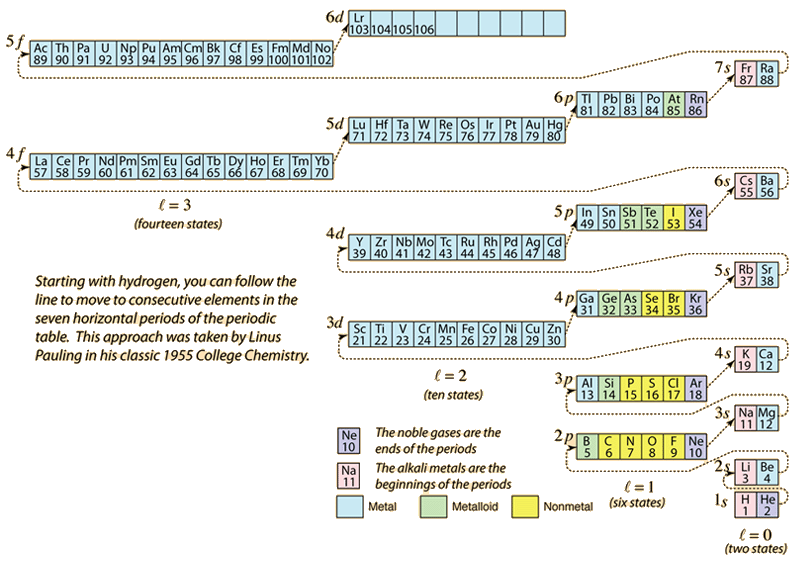
\includegraphics[width=\textwidth]{Q13/images/FyldningAfSkaller2.png}
        \caption{De forskellige orbitaler er her vist liggende i rækkefølge efter deres respektive energi (not to scale).}
        \label{fig:Q13_FyldningAfSkaller2}
    \end{subfigure}
    \caption{Opfyldning af orbitaler.}
    \label{fig:Q13_FyldningAfSkaller}
\end{figure}

\begin{figure}[!h]
    \centering
    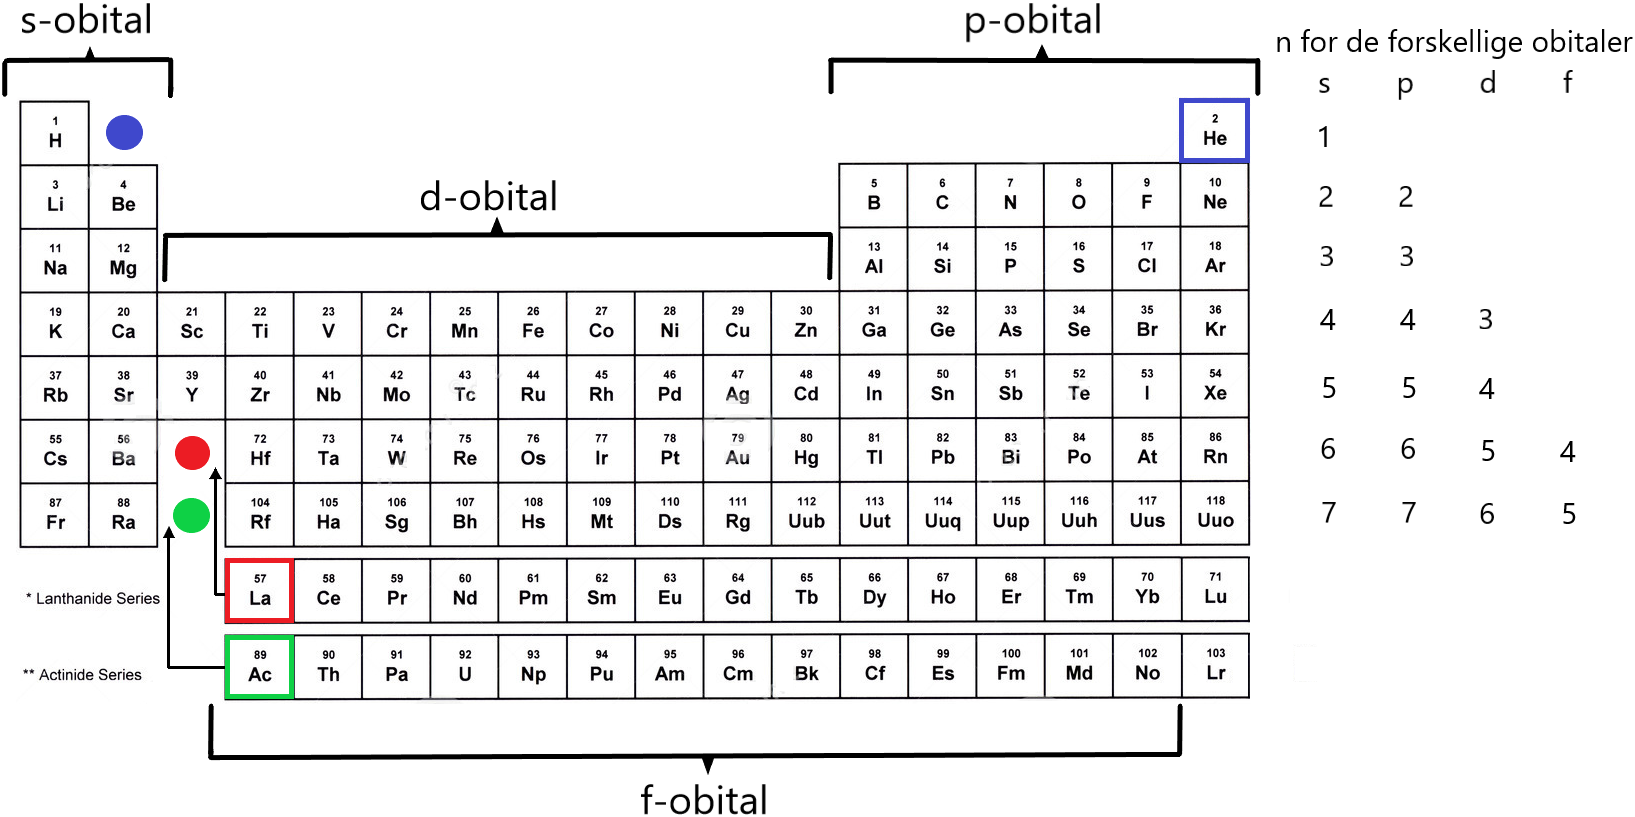
\includegraphics[width=\textwidth]{Q13/images/PeriodicTable.png}
    \caption{\cref{fig:Q13_FyldningAfSkaller} kan også visualiseres direkte i det periodiske system. Her kan det tydeligt ses, at man ikke kan se en række i det periodiske system som opfyldningen af én enkelt skal.}
    \label{fig:Q13_OpfyldningAfSkallerMedPeriodiskSystem}
\end{figure}
$ $\\\\

\paragraph{Generelt om det periodiske system:}
\begin{itemize}
    \item Det periodeske system er arrangeret efter protonnummeret $Z$, hvilket for et ikke ioniseret atom også vil være lig antallet af elektroner.
    \item Herefter er atomerne inddelt i hovedgrupper (1-8), afhængig af Hunds regel, som sørger for, at hver gruppe har lige mange valenselektroner (elektroner i yderste skal), f.eks. har alkalimetaller kun 1 valenselektron, hvorfor de ligger i hovedgruppe 1.
    \begin{itemize}
        \item Fra række 3 findes der mellem hovedgruppe 2 og 3 undergrupperne I-X.
    \end{itemize}
    \item Herefter er grundstofferne også inddelt i 7 rækker, også kaldet skaller, som for s- og p-orbitaler stemmer overens med hovedkvantetallet $n$, og som for d-orbitaler er foskudt med én, således at 3d-orbitalerne ligger i række 4, mens det for f-orbitalerne er forkudt med to, således at 4f-orbitalerne ligger i række 6.
\end{itemize}


\newpage

\begin{figure}[!h]
    \centering
    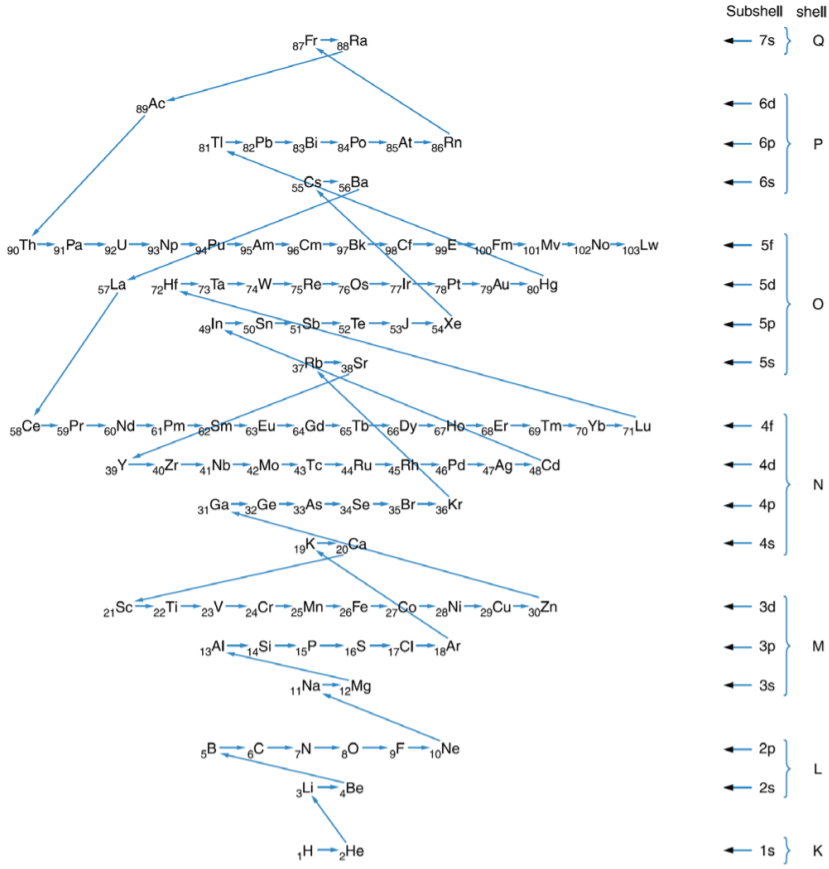
\includegraphics[width=\textwidth]{Q13/images/FyldningAfSkaller.PNG}
    \caption{Faktisk opfyldning af orbitaler, hvilket stort set, med kun få undtagelser, er det samme som vist i \cref{fig:Q13_FyldningAfSkaller}.}
    \label{fig:Q13_FyldningAfSkallerFaktisk}
\end{figure}